\section{Linear combinations}
\label{sec:linear-combinations-rn}

\begin{outcome}
  \begin{enumerate}
  \item Compute linear combinations of vectors algebraically and
    geometrically.
  \item Determine whether a vector is a linear combination of given
    vectors.
  \item Find the coefficients of one vector as a linear combination of
    other vectors.
  \end{enumerate}
\end{outcome}


Now that we have studied both vector addition and scalar
multiplication, we can combine the two operations. You may remember
that when we talked about the solutions to homogeneous systems of
equations in Section~\ref{sec:homogeneous-systems}, we briefly
mentioned that the general solution of a homogeneous system is a
linear combination of its basic solutions. We now return to the
concept of a linear combination.

\begin{definition}{Linear combination}{linear-combination}
  A vector $\vect{v}$ is said to be a \textbf{linear
    combination}\index{linear combination} of the vectors
  $\vect{u}_1,\cdots , \vect{u}_n $ if there exist scalars,
  $a_{1},\cdots ,a_{n}$ such that
  \begin{equation*}
    \vect{v} = a_1 \vect{u}_1 + \ldots + a_n \vect{u}_n.
  \end{equation*}
  The numbers $a_1,\ldots,a_n$ are called the
  \textbf{coefficients}\index{coefficients of a linear combination}\index{linear combination!coefficients}
  of the linear combination.
\end{definition}

\begin{example}{Linear combination}{linear-combination}
  We have
  \begin{equation*}
    3
    \begin{mymatrix}{r}
      -4 \\
      1 \\
      0
    \end{mymatrix}
    +
    2
    \begin{mymatrix}{r}
      -3 \\
      0\\
      1
    \end{mymatrix}
    =
    \begin{mymatrix}{r}
      -18 \\
      3 \\
      2
    \end{mymatrix}. 
  \end{equation*}
  Thus we can say that
  \begin{equation*}
    \vect{v}= \begin{mymatrix}{r}
      -18 \\
      3 \\
      2
    \end{mymatrix}
  \end{equation*}
  is a linear combination of the vectors 
  \begin{equation*}
    \vect{u}_1 = \begin{mymatrix}{r}
      -4 \\
      1 \\
      0
    \end{mymatrix}
    \quad\mbox{and}\quad
    \vect{u}_2 = 
    \begin{mymatrix}{r}
      -3 \\
      0\\
      1
    \end{mymatrix}.
  \end{equation*}
\end{example}

For the specific case of $\R^3$, there are three special vectors which
we often use.  They are given by
\begin{equation*}
\vect{i} = 
\begin{mymatrix}{c}
1 \\ 0 \\ 0
\end{mymatrix},
\quad
\vect{j} = 
\begin{mymatrix}{c}
0 \\ 1 \\ 0
\end{mymatrix},
\quad\mbox{and}\quad
\vect{k} = 
\begin{mymatrix}{c}
0 \\ 0 \\ 1
\end{mymatrix}.
\end{equation*}
We can write any vector $\vect{u} = \mat{a_1,a_2,a_3}^T$ as a linear
combination of these vectors, namely
\begin{equation*}
  \vect{u} = a_1 \vect{i} + a_2 \vect{j} + a_3 \vect{k}.
\end{equation*}
We will use this notation from time to time.

\begin{example}{Determining if linear combination}{determine-lin-comb}
  Can $\vect{v}=\mat{1, 3, 5 }^T$ be written as a linear combination
  of $\vect{u}_1=\mat{2, 2, 6 }^T$, $\vect{u}_2=\mat{1, 6, 8 }^T$, and
  $\vect{u}_3=\mat{3, 8, 18 }^T$? If yes, find the coefficients.
\end{example}

\begin{solution}
  This question can be rephrased as: can we find scalars $x,y,z$ such
  that
  \begin{equation*}
    x\vect{u}_1+y\vect{u}_2+z\vect{u}_3=\vect{v}?
  \end{equation*}
  Multiplying out produces the system of linear equations
  \begin{align*}
    2x+y+3z&=1\\
    2x+6y+8z&=3\\
    6x+8y+18z&=5.
  \end{align*}
  Now we row reduce the corresponding augmented matrix to solve.
  \begin{align*}
    &\begin{mymatrix}{rrr|r} 2 & 1 & 3 & 1 \\ 2 & 6 & 8 & 3\\ 6 & 8 & 18 & 5 \end{mymatrix}
    \stackrel{R_1\leftarrow R_1-R_2}{\stackrel{R_3\leftarrow R_3-3R_1}{\sim}}
    \begin{mymatrix}{rrr|r} 0 & -5 & -5 & -2 \\ 2 & 6 & 8 & 3 \\ 0 & 5 & 9 & 2 \end{mymatrix}
    \stackrel{R_1\leftarrow R_1+R_3}{\sim}
    \begin{mymatrix}{rrr|r} 0 & 0 & 4 & 0 \\ 2 & 6 & 8 & 3 \\ 0 & 5 & 9 & 2 \end{mymatrix}
    \stackrel{R_2\leftrightarrow R_1}{\sim} \\
    &\begin{mymatrix}{rrr|r} 2 & 6 & 8 & 3 \\ 0 & 0 & 4 & 0 \\ 0 & 5 & 9 & 2 \end{mymatrix}
    \stackrel{\frac{1}{2}R_1}{\stackrel{R_2\leftrightarrow R_3}{\sim}}
    \begin{mymatrix}{rrr|r} 1 & 3 & 4 & \frac{3}{2} \\ 0 & 5 & 9 & 2\\  0 & 0 & 4 & 0\end{mymatrix}
    \stackrel{\frac{1}{4}R_3}{\sim}
    \begin{mymatrix}{rrr|r} 1 & 3 & 4 & \frac{3}{2} \\ 0 & 5 & 9 & 2\\  0 & 0 & 1 & 0 \end{mymatrix}
    \stackrel{R_1\leftarrow R_1-4R_3}{\stackrel{R_2\leftarrow R_2-9R_3}{\sim}} \\
    &\begin{mymatrix}{rrr|r} 1 & 3 & 0 & \frac{3}{2} \\ 0 & 5 & 0 & 2\\  0 & 0 & 1 & 0 \end{mymatrix}
    \stackrel{\frac{1}{5}R_2}{\sim}
    \begin{mymatrix}{rrr|r} 1 & 3 & 0 & \frac{3}{2} \\ 0 & 1 & 0 & \frac{2}{5}\\  0 & 0 & 1 & 0 \end{mymatrix}
    \stackrel{R_1\leftarrow R_1-3R_2}{\sim}
    \begin{mymatrix}{rrr|r} 1 & 0 & 0 & \frac{3}{10} \\ 0 & 1 & 0 & \frac{2}{5}\\  0 & 0 & 1 & 0 \end{mymatrix}.
  \end{align*}
  We are in the case where we have a unique solution:
  \begin{align*}
    x&=\frac{3}{10}\\
    y&=\frac{2}{5}\\
    z&=0.
  \end{align*}
  This means that $\vect{v}$ is a linear combination of $\vect{u}_1$,
  $\vect{u}_2$, and $\vect{u}_3$:
  \begin{equation*}
    \vect{v}=\frac{3}{10}\vect{u}_1+\frac{2}{5}\vect{u}_2+0\vect{u}_3.
  \end{equation*}
  The coefficients are $\frac{3}{10}$, $\frac{2}{5}$, and $0$.
  In fact, $\vect{v}$ is also a linear combination of just $\vect{u}_1$ and
  $\vect{u}_2$.
\end{solution}

In the following example, we examine the geometric meaning of linear combinations.

\begin{example}{Graphing a linear combination of vectors}{graphing-linear-combination}
Consider the following picture of the vectors $\vect{u}$ and $\vect{v}$
\begin{center}
\begin{tikzpicture}[scale=2]
\draw[->, thick, blue] (0,0) -- node[above]{$\vect{u}$} (2,1);
\draw[->, thick, red] (4,1) -- node[above]{$\vect{v}$} (5,0.5);
\end{tikzpicture}
\end{center}
Sketch a picture of $\vect{u}+2\vect{v}$ and $\vect{u}-\frac{1}{2}\vect{v}.$
\end{example}

\begin{solution}
Both vectors are shown below.
\begin{center}
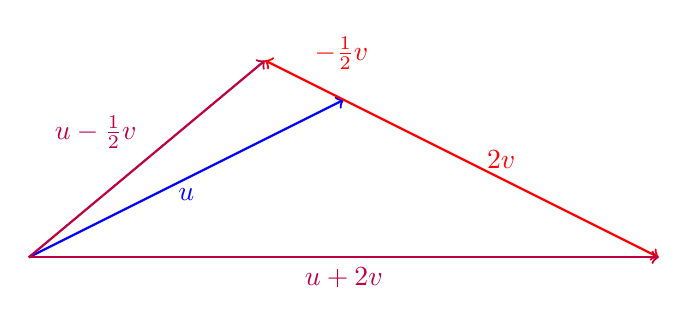
\begin{tikzpicture}[scale=2]
\draw[->, thick, blue] (0,0) -- node[below]{$\vect{u}$} (2,1);
\draw[->, thick, red] (2,1) -- node[above]{$\vect{2v}$} (4,0);
\draw[->, thick, purple](0,0) -- node[below]{$\vect{u}+2\vect{v}$} (4,0);
\draw[->, thick, red] (2,1) -- node[above right]{$-\frac{1}{2}\vect{v}$} (1.5, 1.25);
\draw[->, thick, purple](0,0) -- node[above left]{$\vect{u} - \frac{1}{2}\vect{v}$} (1.5,1.25);
\end{tikzpicture}
\end{center}
\end{solution}

Given any two non-parallel vectors $\vect{u}$ and $\vect{v}$ in
$\R^2$, we can create a grid of their linear combinations. The integer
ones are pictured below. From this we can see that all vectors in
$\R^2$ can be written as a linear combination of $\vect{u}$ and
$\vect{v}$. 

\begin{center}
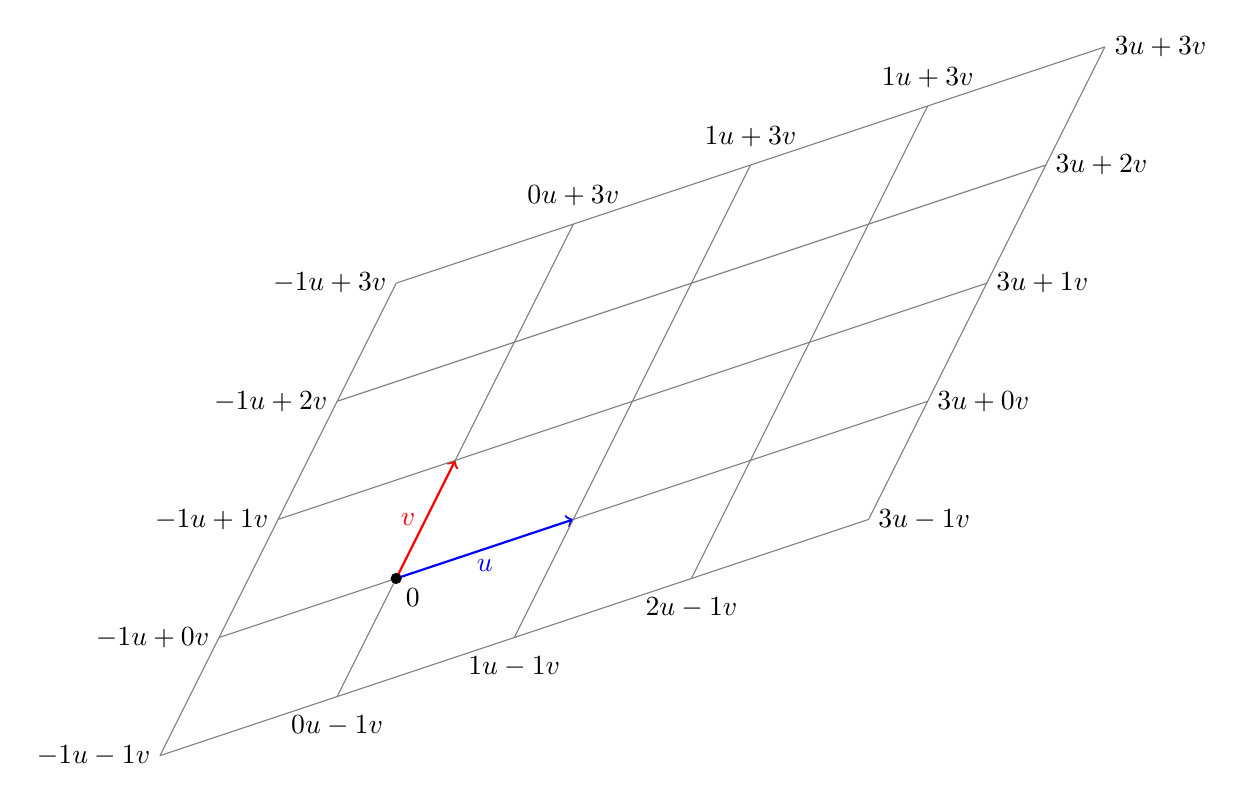
\begin{tikzpicture}[scale=1.5]
\draw[->, thick, blue] (0,0) -- node[below]{$\vect{u}$} (1.5,0.5);
\draw[->, thick, red] (0,0) -- node[left]{$\vect{v}$} (0.5,1);
\draw[-, gray] (-2,-1.5)--(4,0.5);
\draw[-, gray] (-1.5,-0.5)--(0,0);
\draw[-, gray] (1.5,0.5)--(4.5,1.5);
\draw[-, gray] (-1,0.5)--(5,2.5);
\draw[-, gray] (-0.5,1.5)--(5.5,3.5);
\draw[-, gray] (0,2.5)--(6,4.5);
\draw[-, gray] (-2,-1.5)--(0,2.5);
\draw[-, gray] (-0.5,-1)--(0,0);
\draw[-, gray] (0.5,1)--(1.5,3);
\draw[-, gray] (1,-0.5)--(3,3.5);
\draw[-, gray] (2.5,0)--(4.5,4);
\draw[-, gray] (4,0.5)--(6,4.5);
\draw (-2.0,-1.5) node[left]{$-1\vect{u}-1\vect{v}$};
\draw (-1.5,-0.5) node[left]{$-1\vect{u}+0\vect{v}$};
\draw (-1.0,0.5) node[left]{$-1\vect{u}+1\vect{v}$};
\draw (-0.5,1.5) node[left]{$-1\vect{u}+2\vect{v}$};
\draw (0.0,2.5) node[left]{$-1\vect{u}+3\vect{v}$};
\draw (1.5,3.0) node[above=0.75ex]{$0\vect{u}+3\vect{v}$};
\draw (3.0,3.5) node[above=0.75ex]{$1\vect{u}+3\vect{v}$};
\draw (4.5,4.0) node[above=0.75ex]{$1\vect{u}+3\vect{v}$};
\draw (6.0,4.5) node[right]{$3\vect{u}+3\vect{v}$};
\draw (5.5,3.5) node[right]{$3\vect{u}+2\vect{v}$};
\draw (5.0,2.5) node[right]{$3\vect{u}+1\vect{v}$};
\draw (4.5,1.5) node[right]{$3\vect{u}+0\vect{v}$};
\draw (4.0,0.5) node[right]{$3\vect{u}-1\vect{v}$};
\draw (2.5,0.0) node[below=0.75ex]{$2\vect{u}-1\vect{v}$};
\draw (1.0,-0.5) node[below=0.75ex]{$1\vect{u}-1\vect{v}$};
\draw (-0.5,-1.0) node[below=0.75ex]{$0\vect{u}-1\vect{v}$};
\draw[fill] (0,0) circle [radius=1.2pt] node[below right]{$\vect{0}$};
\end{tikzpicture}
\end{center}
